\section{Simulation}

%\subsection{Expected physics performance}

%A series MC simulation have been used to calculate the acceptance of the central detector and have reconstructed physics parameters for types of events that are of interest. Fig. ... shows the missing mass resolution expected for MC simulation studies for a number of different reactions. For all cases studied, the results show that it is possible to identify the missing particle for each reaction.
%Figure ... shows the missing mass spectrum expected when pion is detected in the central tracker. There is sufficient resolution to study resonant production and to compare, for example, s, t, and u channel processes.

\subsection{Detector simulation}

A realistic model of the SVT has been developed, describing the location and composition of all modules, with material description based on the engineering drawings and assembly procedures, and confirmed by the survey measurements during integration. The SVT design and module layout were validated by Geant-4-based simulated detector performance studies demonstrating compliance with the technical requirements and engineering models. A 3D view of the simulated geometry of the SVT sensors is shown in Fig.~\ref{fig:svt3dview}.    

\begin{figure}[hbt] 
\centering 
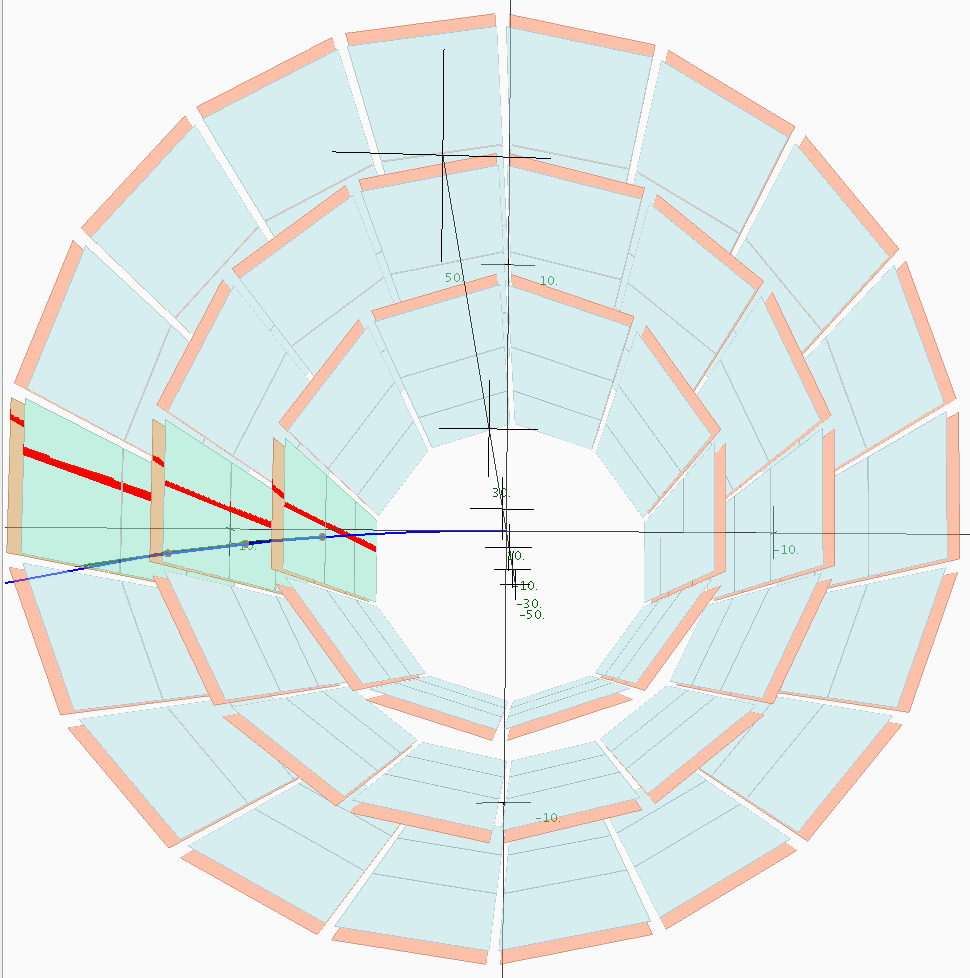
\includegraphics[width=0.6\columnwidth,keepaspectratio]{svt3dview.png}
\caption{3D view of the simulated SVT detector geometry.}
\label{fig:svt3dview}
\end{figure}

\subsection{Backgrounds, energy deposition, dose rates}

Simulations of beam-related backgrounds were performed for several thicknesses of a tungsten shielding cylinder around the CLAS12 target covering the first SVT layer. Rates, fluences, radiation doses, and 1 MeV neutron damage rates in the SVT were calculated for different particles. For each event, 124,000 electrons going through the target within a 248.5-ns time window were simulated. This corresponds to the full CLAS12' $10^{35}$cm$^{-2}$s$^{-1}$ luminosity on a 5-cm-long liquid-hydrogen target at 11 GeV beam energy. Rates in the first SVT layer for a liquid-hydrogen target are shown in Fig.~\ref{fig:rates-lh2}. The energy deposited in layer 1 for the electromagnetic and the hadronic particles is shown in Fig.~\ref{fig:energy-deposited-l1}. At a threshold of 30 keV, 92$\%$ of the electromagnetic background is rejected while preserving  99.5$\%$ of the signals coming from the hadrons~\cite{TDRSVT}.
 
\begin{figure}[hbt] 
\centering 
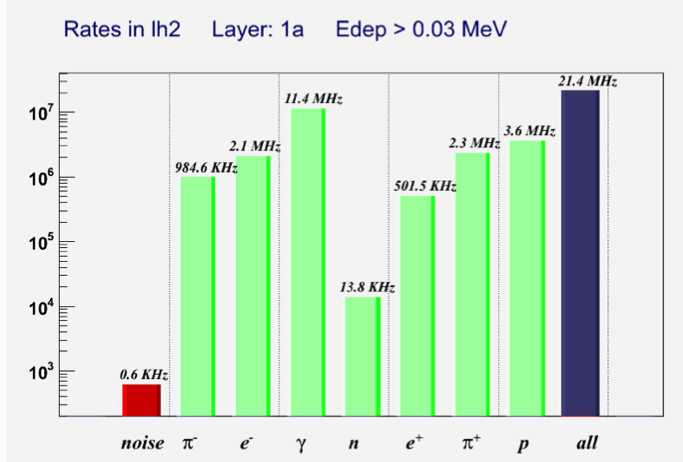
\includegraphics[width=1.0\columnwidth,keepaspectratio]{rates-lh2.png}
\caption{Rates in the first SVT layer for a 5-cm long liquid hydrogen target at the nominal CLAS12 operating luminosity of $10^{35}$cm$^{-2}$s$^{-1}$.}
\label{fig:rates-lh2}
\end{figure}

\begin{figure}[hbt] 
\centering 
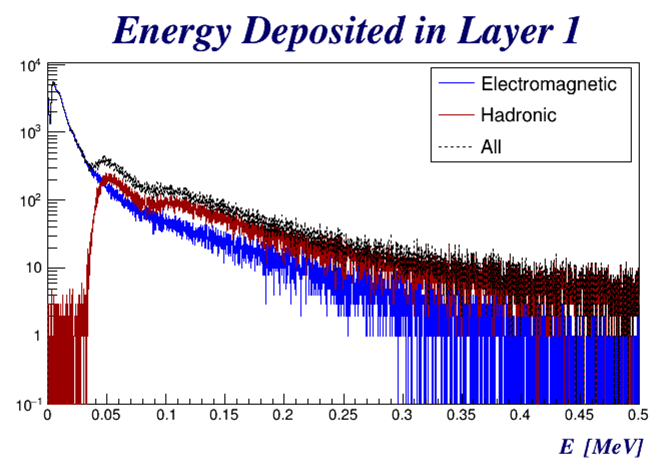
\includegraphics[width=0.8\columnwidth,keepaspectratio]{energy-deposited-l1.png}
\caption{Energy deposited in the SVT layer 1 for electromagnetic and hadronic particles for a liquid hydrogen target at the nominal CLAS12 operating luminosity.}
\label{fig:energy-deposited-l1}
\end{figure}

A tungsten shield 51~$\mu$m thick is installed on the target scattering chamber. The shield consists of 2 sheets mounted over the top and bottom halves of the foam cylinder referenced to the SVT common ground. The SVT rates and radiation damage benefit from the inclusion of the tungsten shield. The rates have been compared with physics run data at several beam currents. There is a good agreement between the real and the simulated data.

While the gamma fluences / doses show a dramatic decrease with the introduction of shielding, the total fluences and doses decrease significantly for the thinner configuration and do not vary much for thicker tungsten (see Fig.~\ref{fig:rates-l1}). The photon radiation dose becomes negligible for 50 $\mu$m or more of tungsten with total 1 MeV equivalent radiation dose about 65 krad per year on a liquid-hydrogen target. For 15 years of running the experiment on a carbon target the estimated radiation dose for the sensors is 2.5~Mrad \cite{TDRSVT}. 

\begin{figure}[hbt] 
\centering 
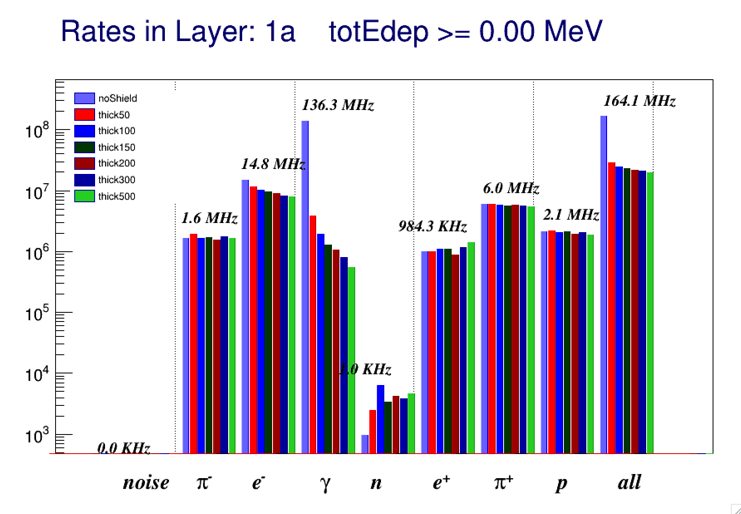
\includegraphics[width=1.0\columnwidth,keepaspectratio]{rates-l1.png}
\caption{Rates in the first SVT layer for different tungsten shield thickness from 50 to 500 $\mu$m for a liquid hydrogen target at the nominal CLAS12 operating luminosity. No energy threshold cut applied.}
\label{fig:rates-l1}
\end{figure}

%\subsection{Occupancies}

%\subsection{Alignment}

%Validation of alignment procedures was performed on Monte Carlo simulation and cosmic data. Detector alignment procedure is using a least squares approach of a Millepede II algorithm \cite{Millepede}. The dependence of the residuals on the track parameters is explicitly taken into account. The alignment code uses the partial derivatives of the distance of closest approach (DOCA) taken with respect to the track parameters and the SVT geometry. This approach accounts for correlated shifts among the geometry parameters. Results of alignment correction for one of the SVT modules are shown in Fig.~\ref{fig:alignment}. Only shifts in the sensor plane were taken into account in the alignment procedure for this plot.

%\begin{wrapfigure}{l}{0.5\columnwidth}
%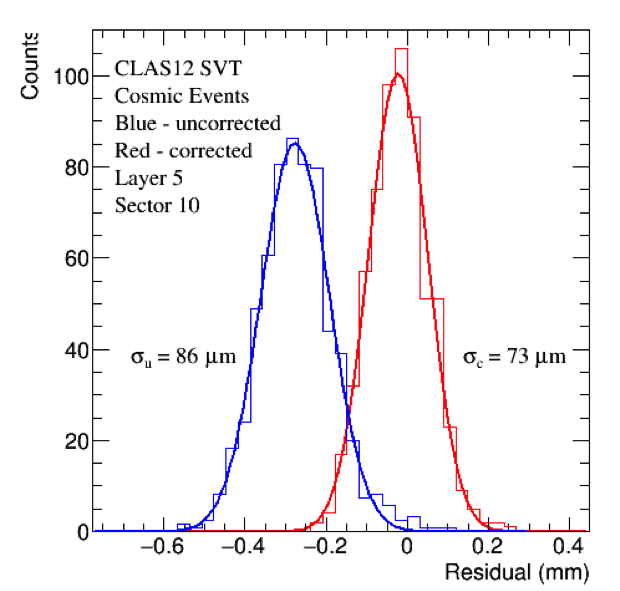
\includegraphics[width=1.0\columnwidth]{alignment.png}
%\caption{Alignment of the SVT module.}
%\label{fig:alignment}
%\end{wrapfigure}

%\subsection{Resolutions}
%
%According to the results of GEANT simulation of the SVT, a resolution of 50~$\mu$m in the bending plane is needed to measure, with a precision better than 5$\%$, tracks with momentum up to 1~GeV (see Fig.~\ref{fig:PtRes}) \cite{MC1,MC2}. 
%
%\begin{wrapfigure}{l}{0.45\columnwidth}
%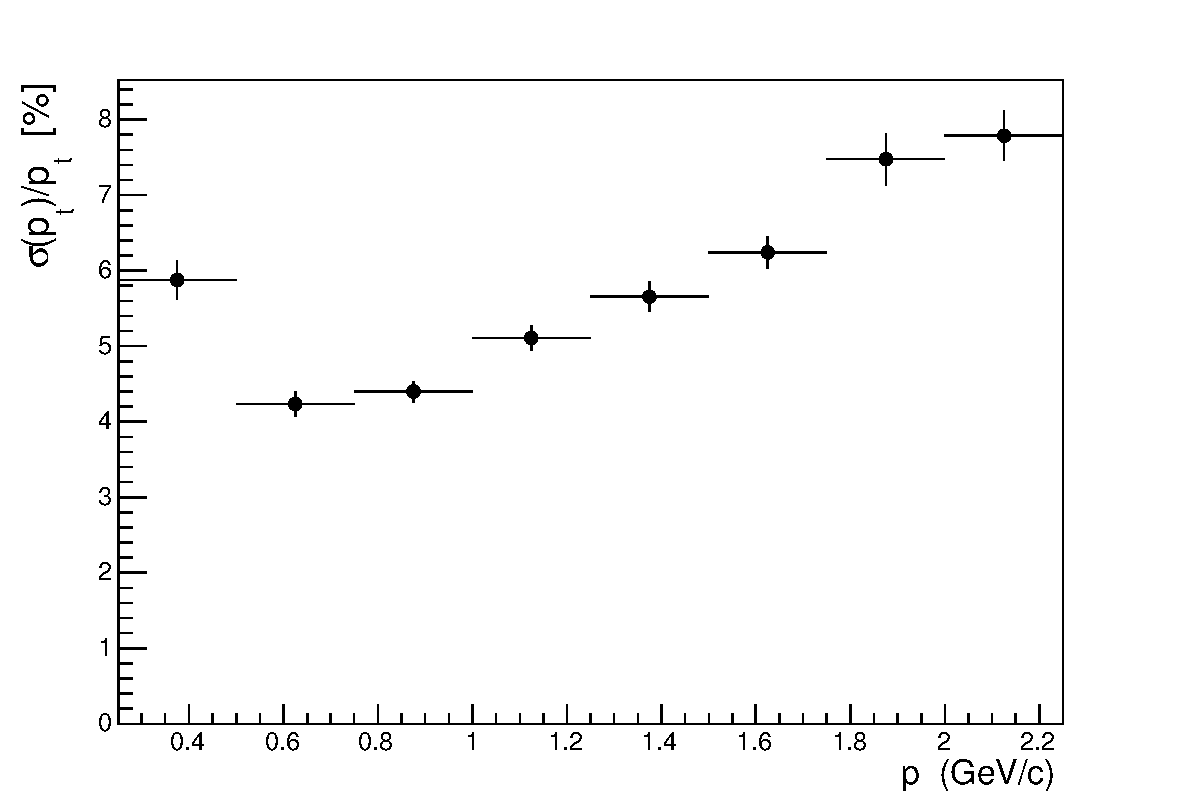
\includegraphics[width=0.45\columnwidth]{PtResol.pdf}
%\caption{Simulated SVT momentum resolution.}
%\label{fig:PtRes}
%\end{wrapfigure}
%
%\subsection{Efficiencies}

